\section{Week 02}

\subsection{27/07/2015}

\textbf{Stage and copy file from CERN servers}

Patrick have copied all the .slcio files in his directory and processed them with Marlin using two bash scripts. We have copied the ntuples from eos (see the glossary) to our folder, and now we can loop among them. 

He used two files: jobCopy.sh and jobMarlin.sh to process the files.

jobCopy first stage the files from the tape (Castor) to the disk, and then copies the files into EOS folder.
jobMarlin loops above all the files writing the correct steering.xml file and create all the ntuple.

\textbf{More about the slcio ntuples}

We have found out something else about our ntuples: 

We discovered that all the top quark have status 3, and the bottoms have sometimes status 2 and sometimes status 3.

By using the parent information (mcpa0 e mcpa1, for daughters mcda0,1,2,3,4) we managed to select only the leptons which come from the W decay. Then, with a pyroot macro we filled the 2-D histograms of the number of leptons versus the energy and the angle.


\subsection{28/07/2015}

\textbf{Lepton vs energy-angle histogram}

We managed to loop above all the .root files. We use 256 bins (16 for the angle and 16 for the energy), that are quite similar to the square root of the entries (they are about 40k, the 40\% of 100k events).\\
We have also used the reduced energy defined as \[x=\frac{2E}{m_t} \sqrt{\frac{1-\beta}{1+\beta}} \]   \[ \beta =\sqrt{1-4m_t^2/s} \]
We plotted the histo of the number of lepton in function of the $cos(\theta)$ and of the reduced energy. We expected a curve distribution in both the variables, and, to do this, we have to plot only the positive leptons (or the negative); otherwise there can't be any asymmetry in the angular distribution.

The result can be seen in figure \ref{02_Electrons}, \ref{02_Muons}, \ref{02_Electrons+muons}

\begin{figure} [ht!]
  \centering
  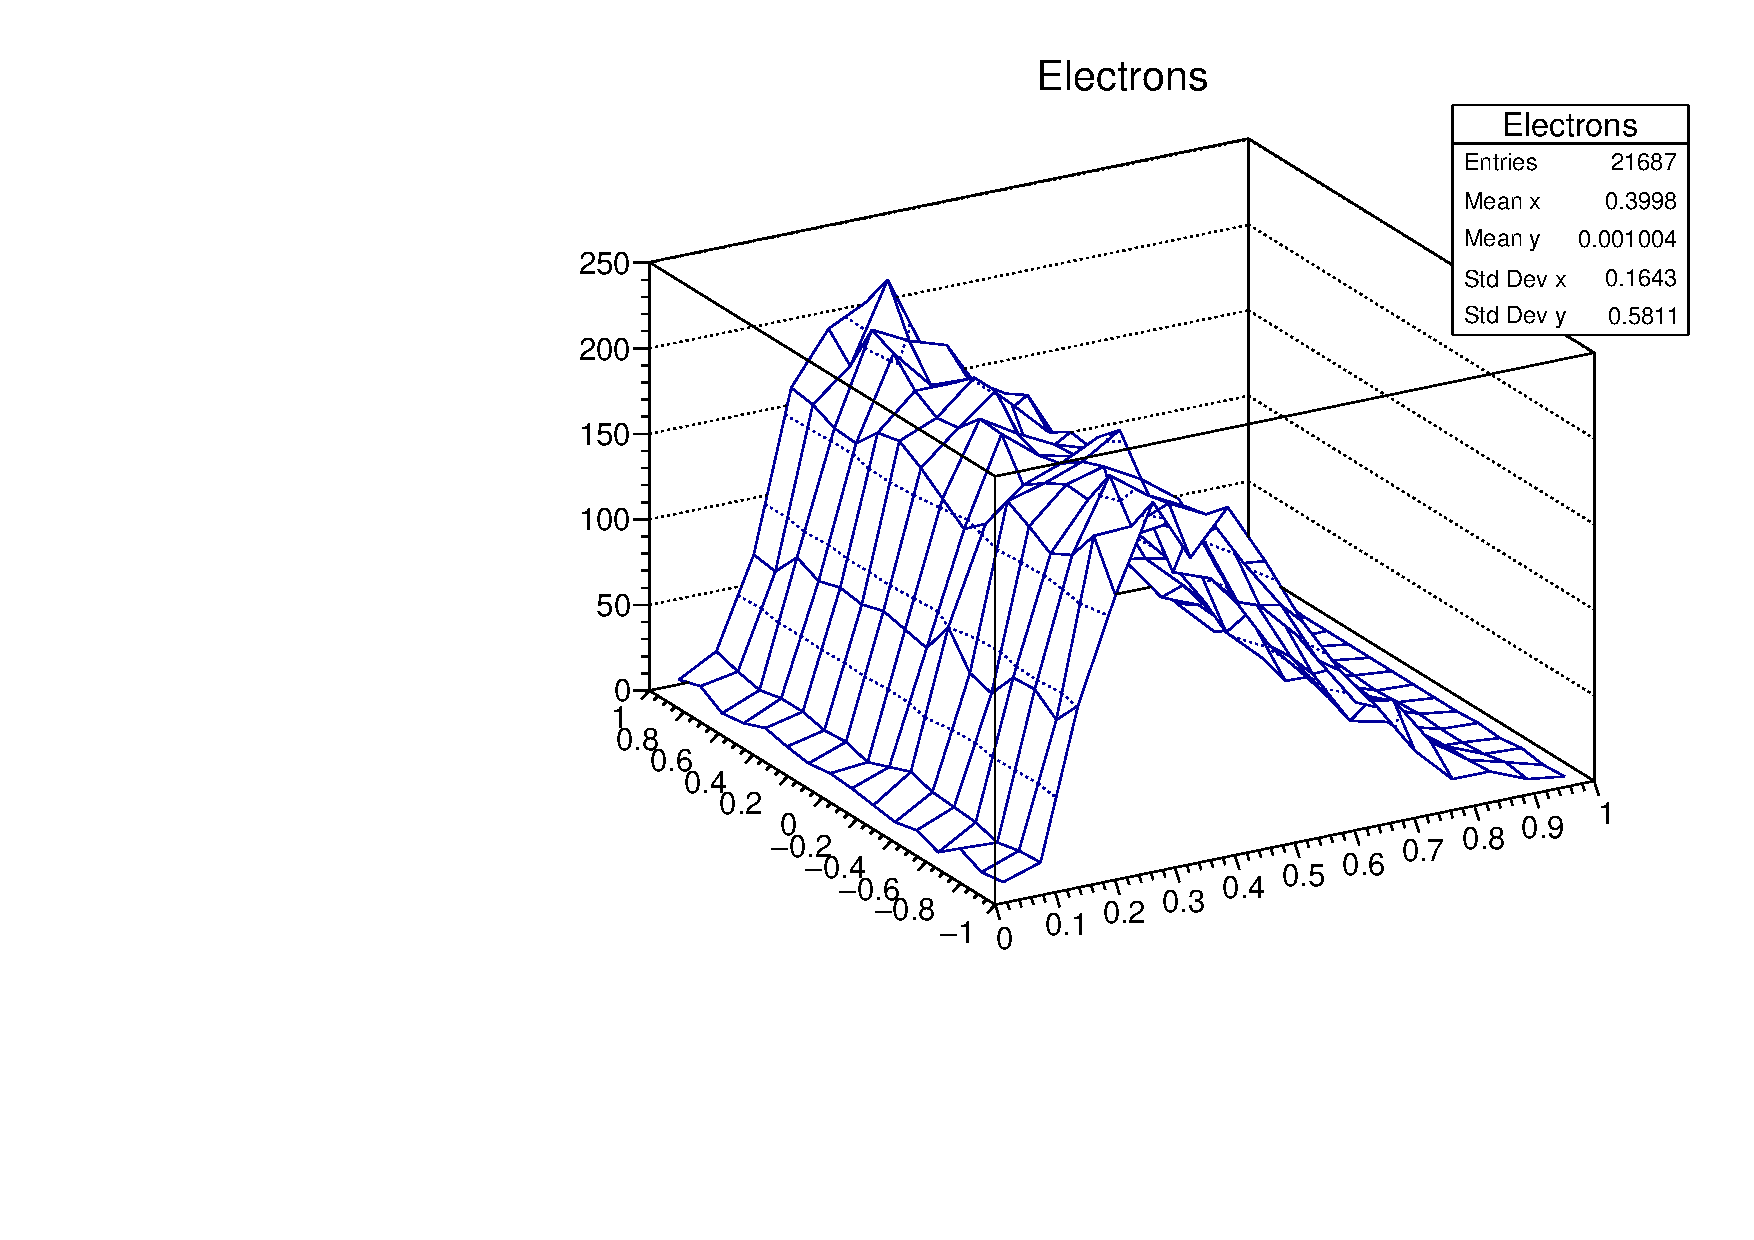
\includegraphics[width=0.7\textwidth]{02_Electrons.pdf}
 \caption{Energy-angle distribution of the electrons}
 \label{02_Electrons}
\end{figure}

\begin{figure} [ht!]
  \centering
  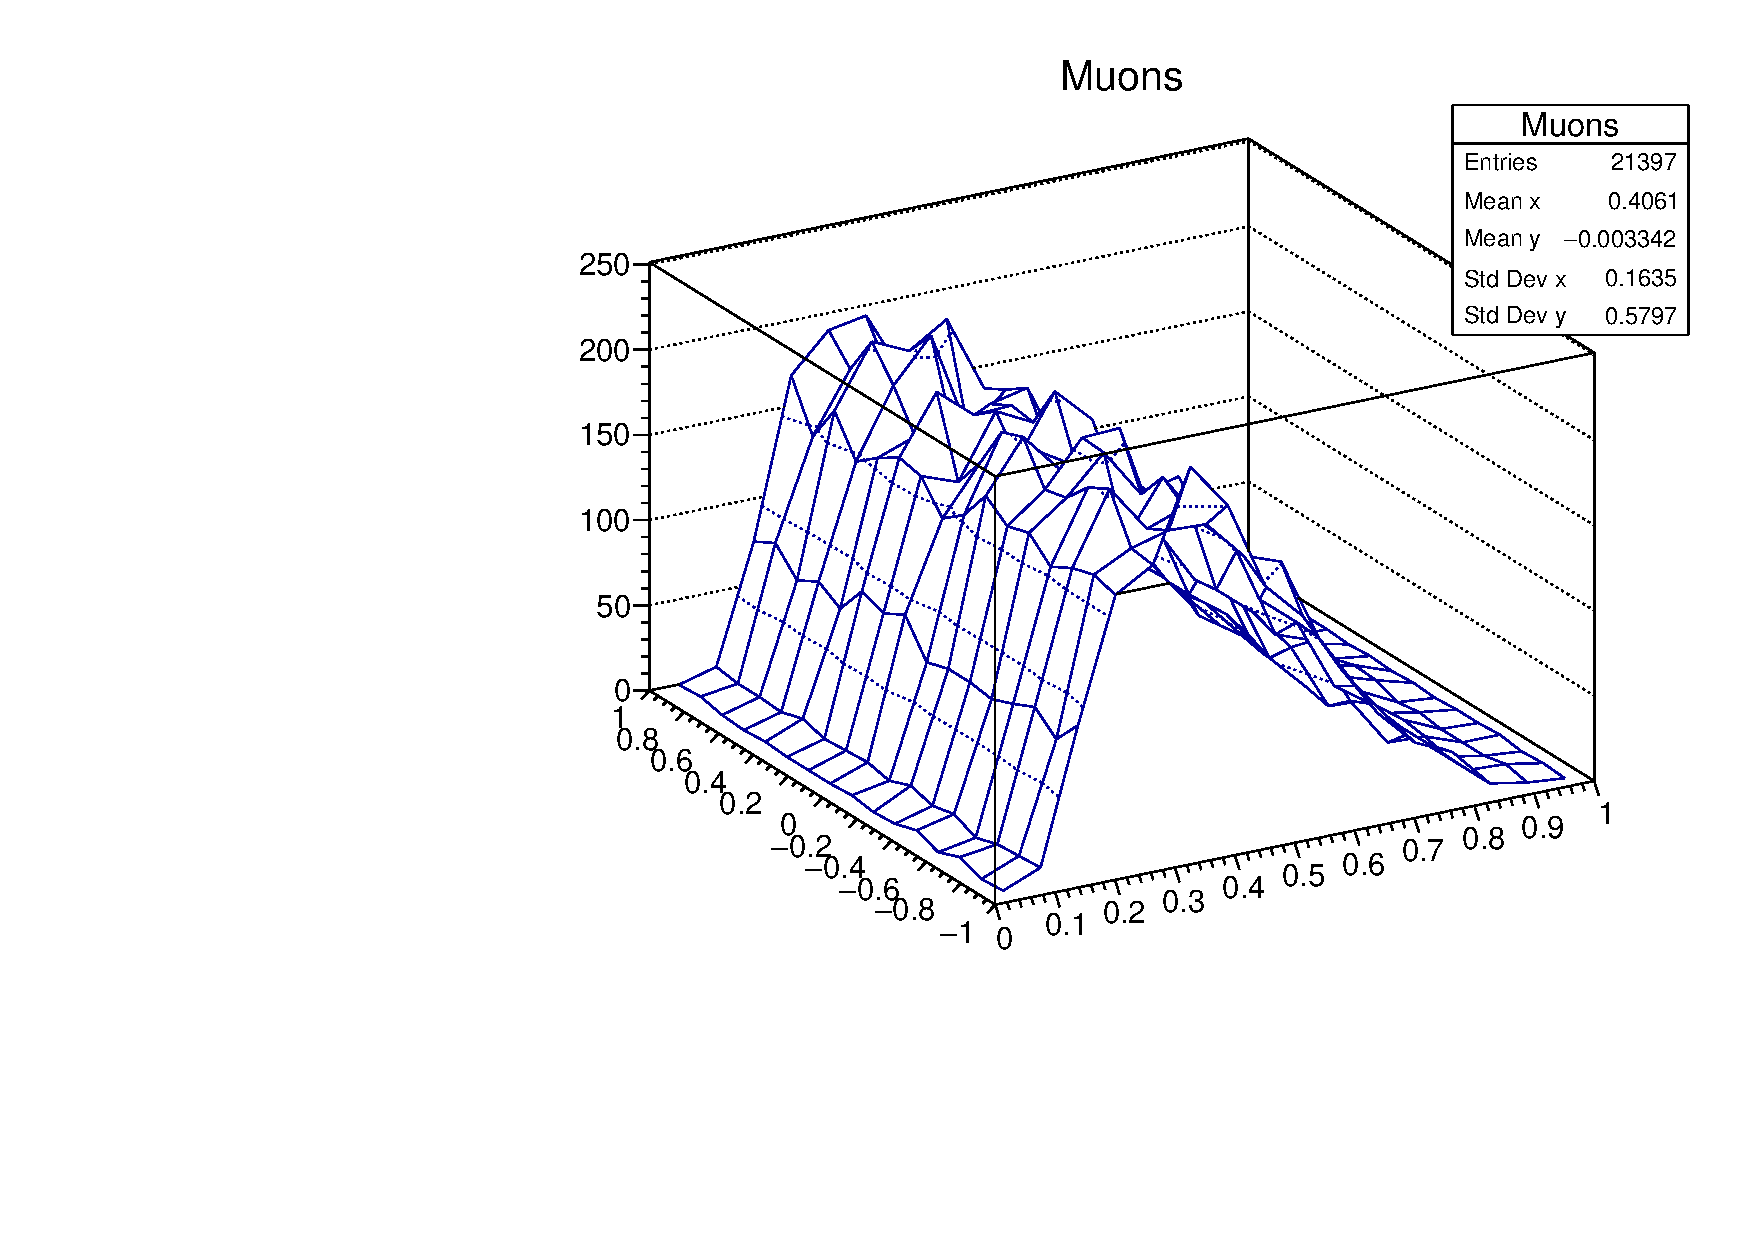
\includegraphics[width=0.7\textwidth]{02_Muons.pdf}
 \caption{Energy-angle distribution of the negative muons}
 \label{02_Muons}
\end{figure}

\begin{figure} [ht!]
  \centering
  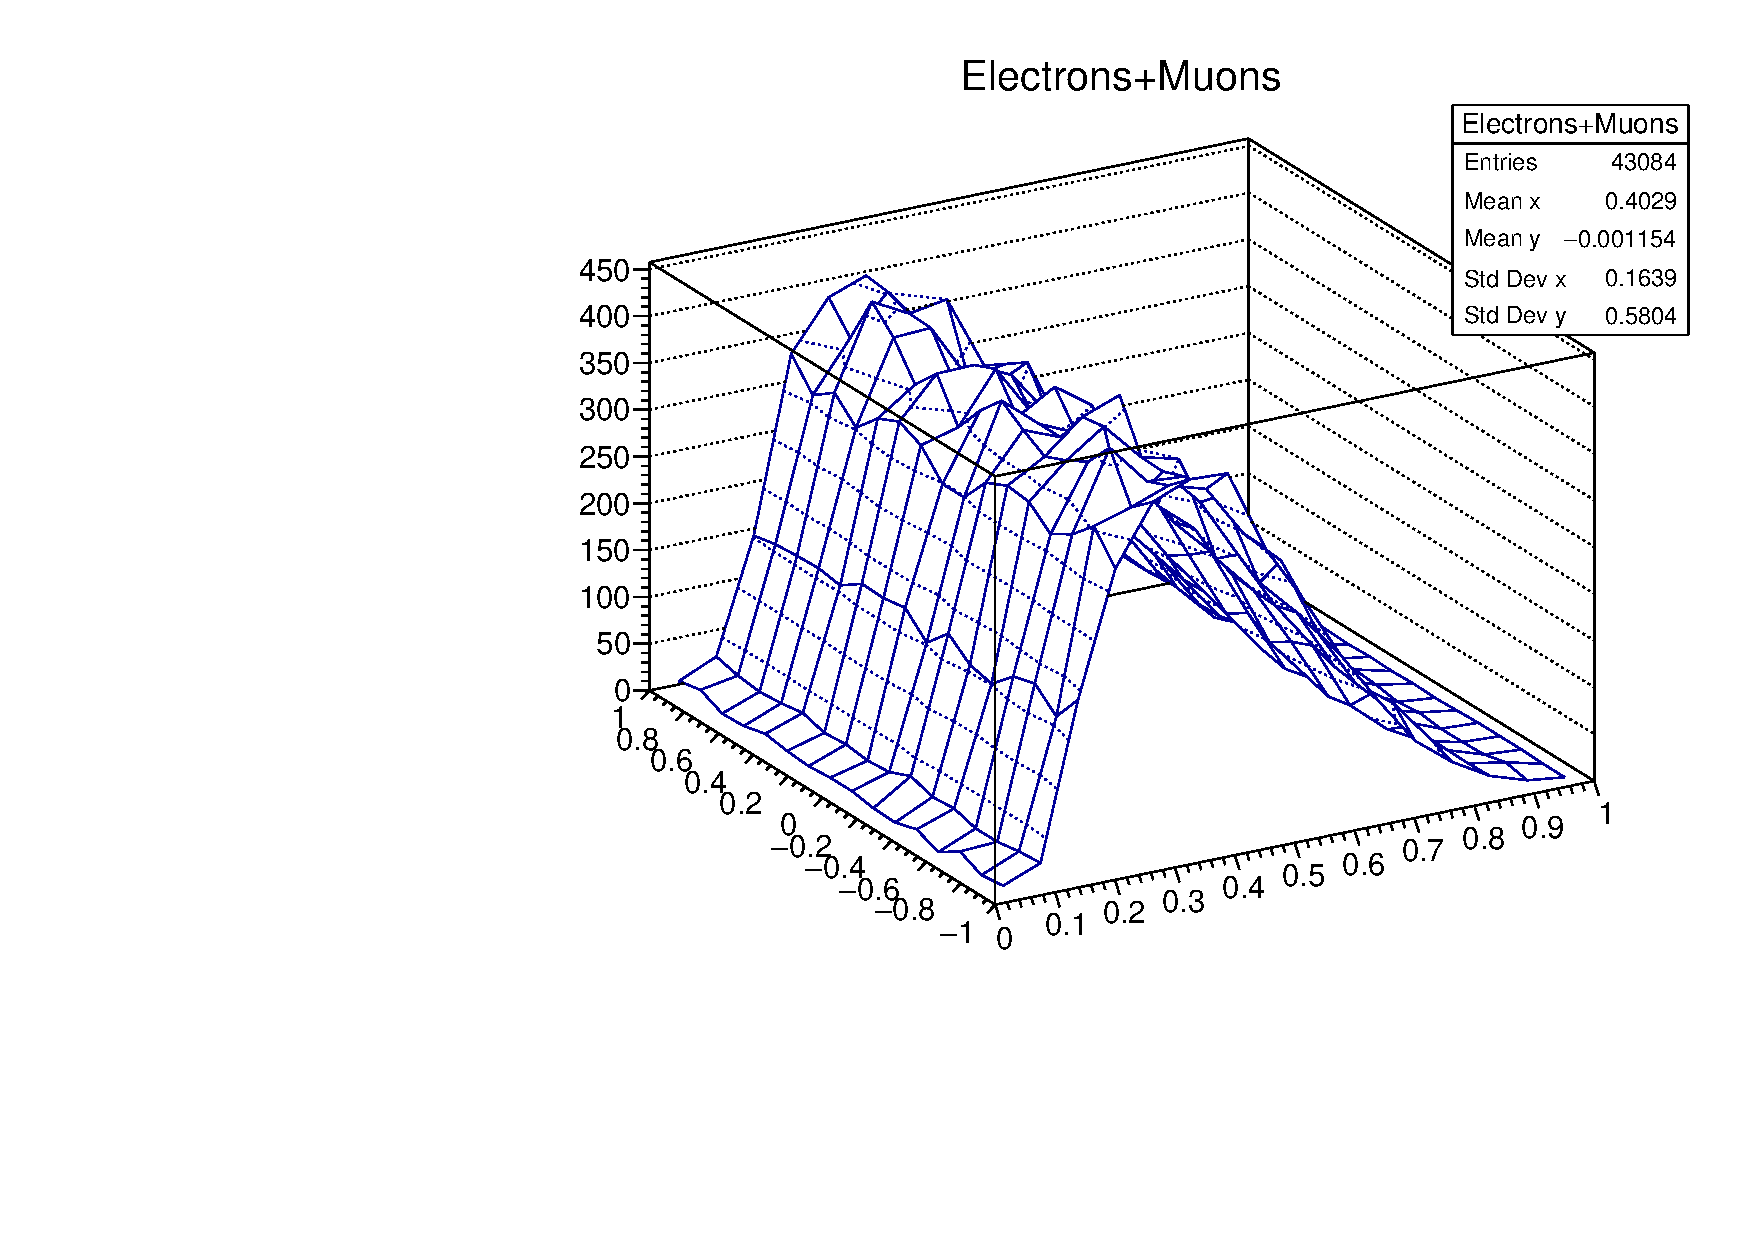
\includegraphics[width=0.7\textwidth]{02_Electrons+muons.pdf}
 \caption{Energy-angle distribution of the electrons and negative muons}
 \label{02_Electrons+muons}
\end{figure}

Unfortunately the angular distribution is flat: this implies that Pythia simulation don't consider the top polarization. So we cannot use these simulation to perform our analysis, and we need to proceed with different data.

\textbf{Writing Root Tree using PyROOT}

We have also learn how to write a Tree Root using PyROOT. We need first to define a TTree variable, then define the branches, and then fill the branches with a 0-D array (this is important), by looping on the events.
Further information in the glossary folder.

\subsection{29/07/2015}

\textbf{Copy and Marlin new simulation files}

We decided to use other simulation files made with Wizard (instead that Pythia), we could find them at this site \href{https://twiki.cern.ch/twiki/bin/view/CLIC/MonteCarloSamplesForTopPhysics?sortcol=2;table=3;up=1#sorted_table.}{clicca qui}
These simulations are made at 365 GeV and would consider the polarization of the top quarks (we hope so).

By using some scripts bash we have staged all the files, copied and Marlin them.